%-------------------------------------------------------------------------------
% File: database.tex
%       Part of StockSim project documentation.
%       See main.tex for further information.
%-------------------------------------------------------------------------------
\chapter{Database}
The database is composed by 8236 stocks from the US stock market, along with
their general information and historical data; the application also needs to
store users and admins login credentials, personal information and the
composition and details of each user's portfolio.\\
We decided to use a column database (Apache Cassandra) for the storage of
historical data; this is because historical data represents almost the 99\%\ of
the entire database and it is going to be growing very fast as days go by;
aggregation and financial analytics on these volumes of data will perform better
in a column database where data storage is designed to optimize this type of
operations by column.\\
We decided to store any other information using a document database (MongoDB),
in order to exploit the schemaless property to save memory; data frequently
needed together is stored in the same document and indexes were created to speed
up linking between documents; 

\section{Dataset}
The initial set of data was fetched from the web, by means of Python scripts using
\texttt{pandas}, \texttt{yfinance} and \texttt{JSON} as support libraries and
relying upon \url{www.nasdaqtrader.com} and \url{finance.yahoo.com}.
\subsection{NasdaqTrader}
The Nasdaq Stock Market (Nasdaq) is the largest U.S. equities exchange venue by volume. 
\footnote{https://www.nasdaqtrader.com/} \\
We choose to take our set of stocks from the Nasdaq index, because it is very popular and
includes a large number of stock, representative of different economy sectors. This will allow 
users to interact with big and famous companies stocks (like Google, Apple, Tesla...), but also
to try smaller companies and/or minor sectors investments. 
NasdaqTrader provides us a stock symbols' list of all the stocks entered in the NASDAQ index
from 1970 until now;
\subsection{Yahoo! Finance}
"Yahoo Finance provides free stock quotes, up-to-date news, portfolio management resources, 
international market data, social interaction and mortgage rates that help you manage your 
financial life." \footnote{https://finance.yahoo.com/} \\
Yahoo Finance is a service, been part of the Yahoo network, that provides several of information
about stocks and companies; they are frequently updated, reliable and well organized.\\
We decided to use this service to retrieve the starting dataset of stocks; we extract only 
the fields that we need, and parse into a JSON file. In this way  it
is possible to rebuild from scratch this dataset into MongoDB with few commands (including
mongoimport).
With Yahoo Finance it is also possible to retrieve historical data of market values for every 
stocks. Using this service it has been possible to build a dataset of all the market values of
each stocks coming from NasdaqTrader; values are collected daily, and we decided to take all 
the values from 2010 to 2020; this dataset (around 1.43 GB) has been parsed to CVS files and
than imported into a Cassandra Cluster. Thanks to the Yahoo Finance service, it's possible
to update every day the database with the last session results. It's also possible to add a new
stock to the dataset, coming from every market exchange of every country.

\hfill \break
{\centering
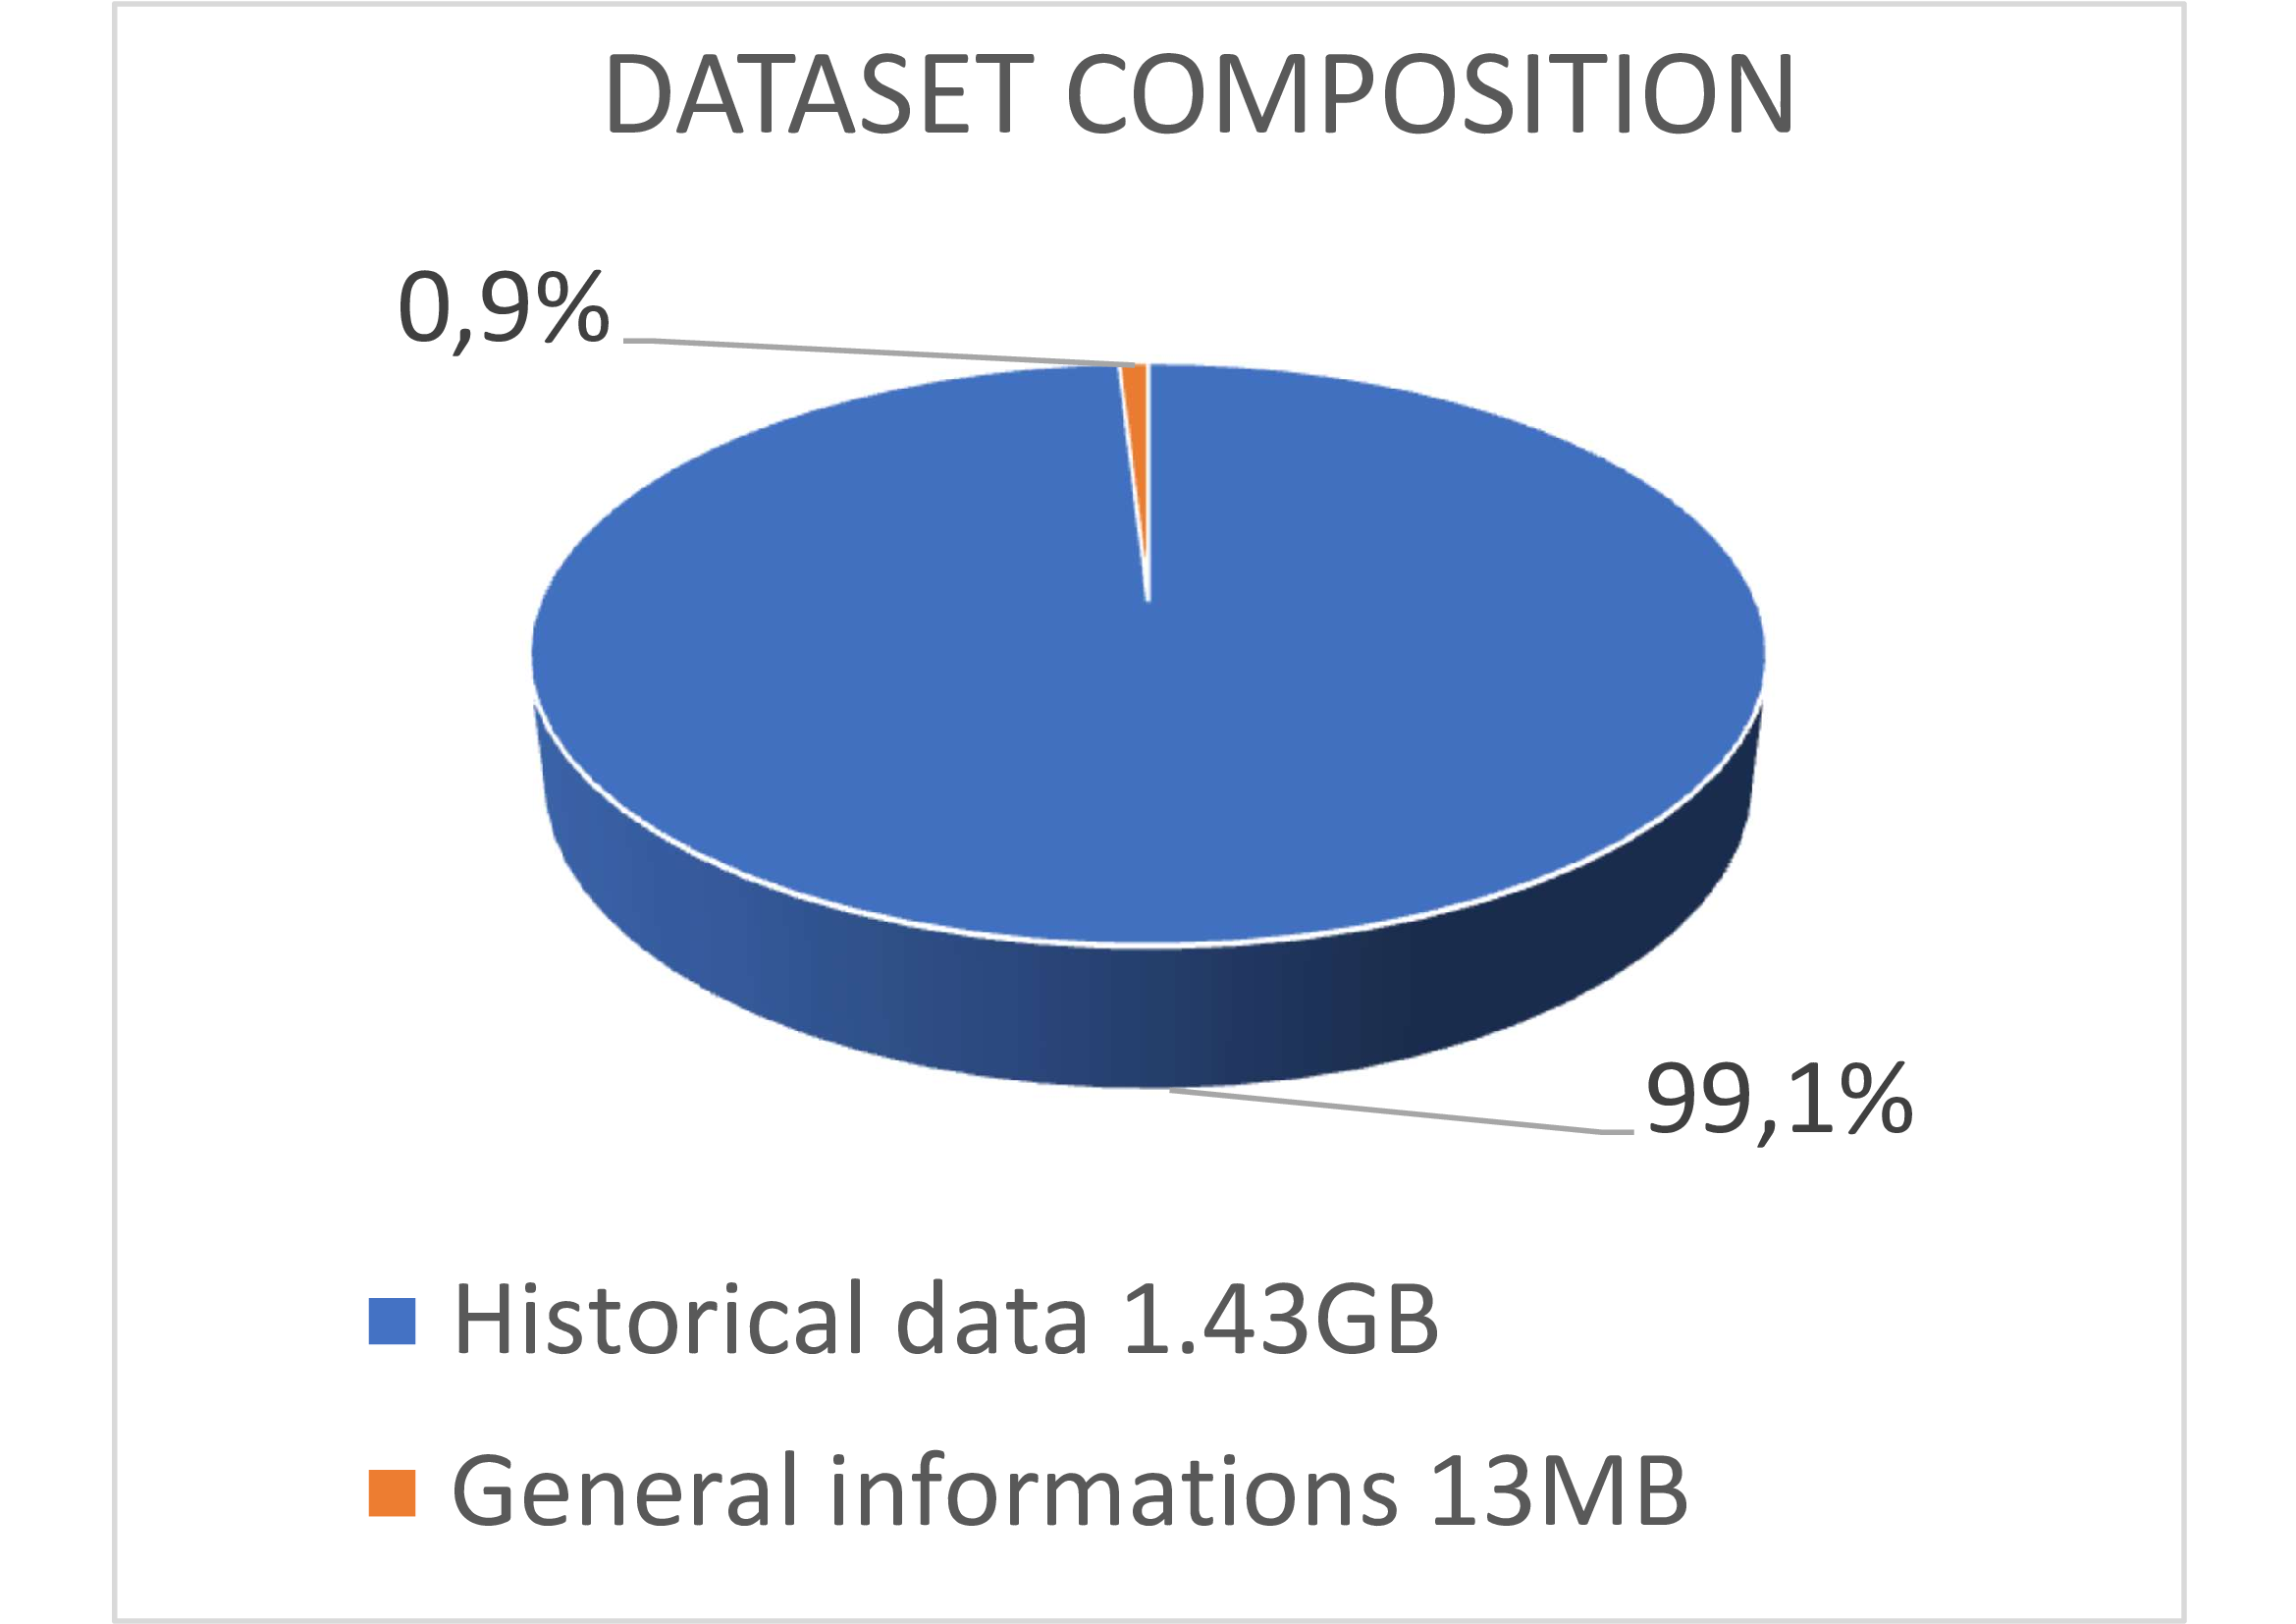
\includegraphics[scale=0.12]{img/dataset_comp.png}\\
}


\section{MongoDB}
"MongoDB is a general purpose, document-based, distributed database build
for modern application developers and for the cloud era." Taken from www.mongodb.com.\\
MongoDB is a very famous document database with a great support for cloud operations, which 
will improve the availability of our application. It also supports several analytic functions
and the creation of custom indexes in order to speedup read operations.
In order to organize data in a meaningful and memory-optimal way, we opted for this structure:

\hfill \break
{\centering
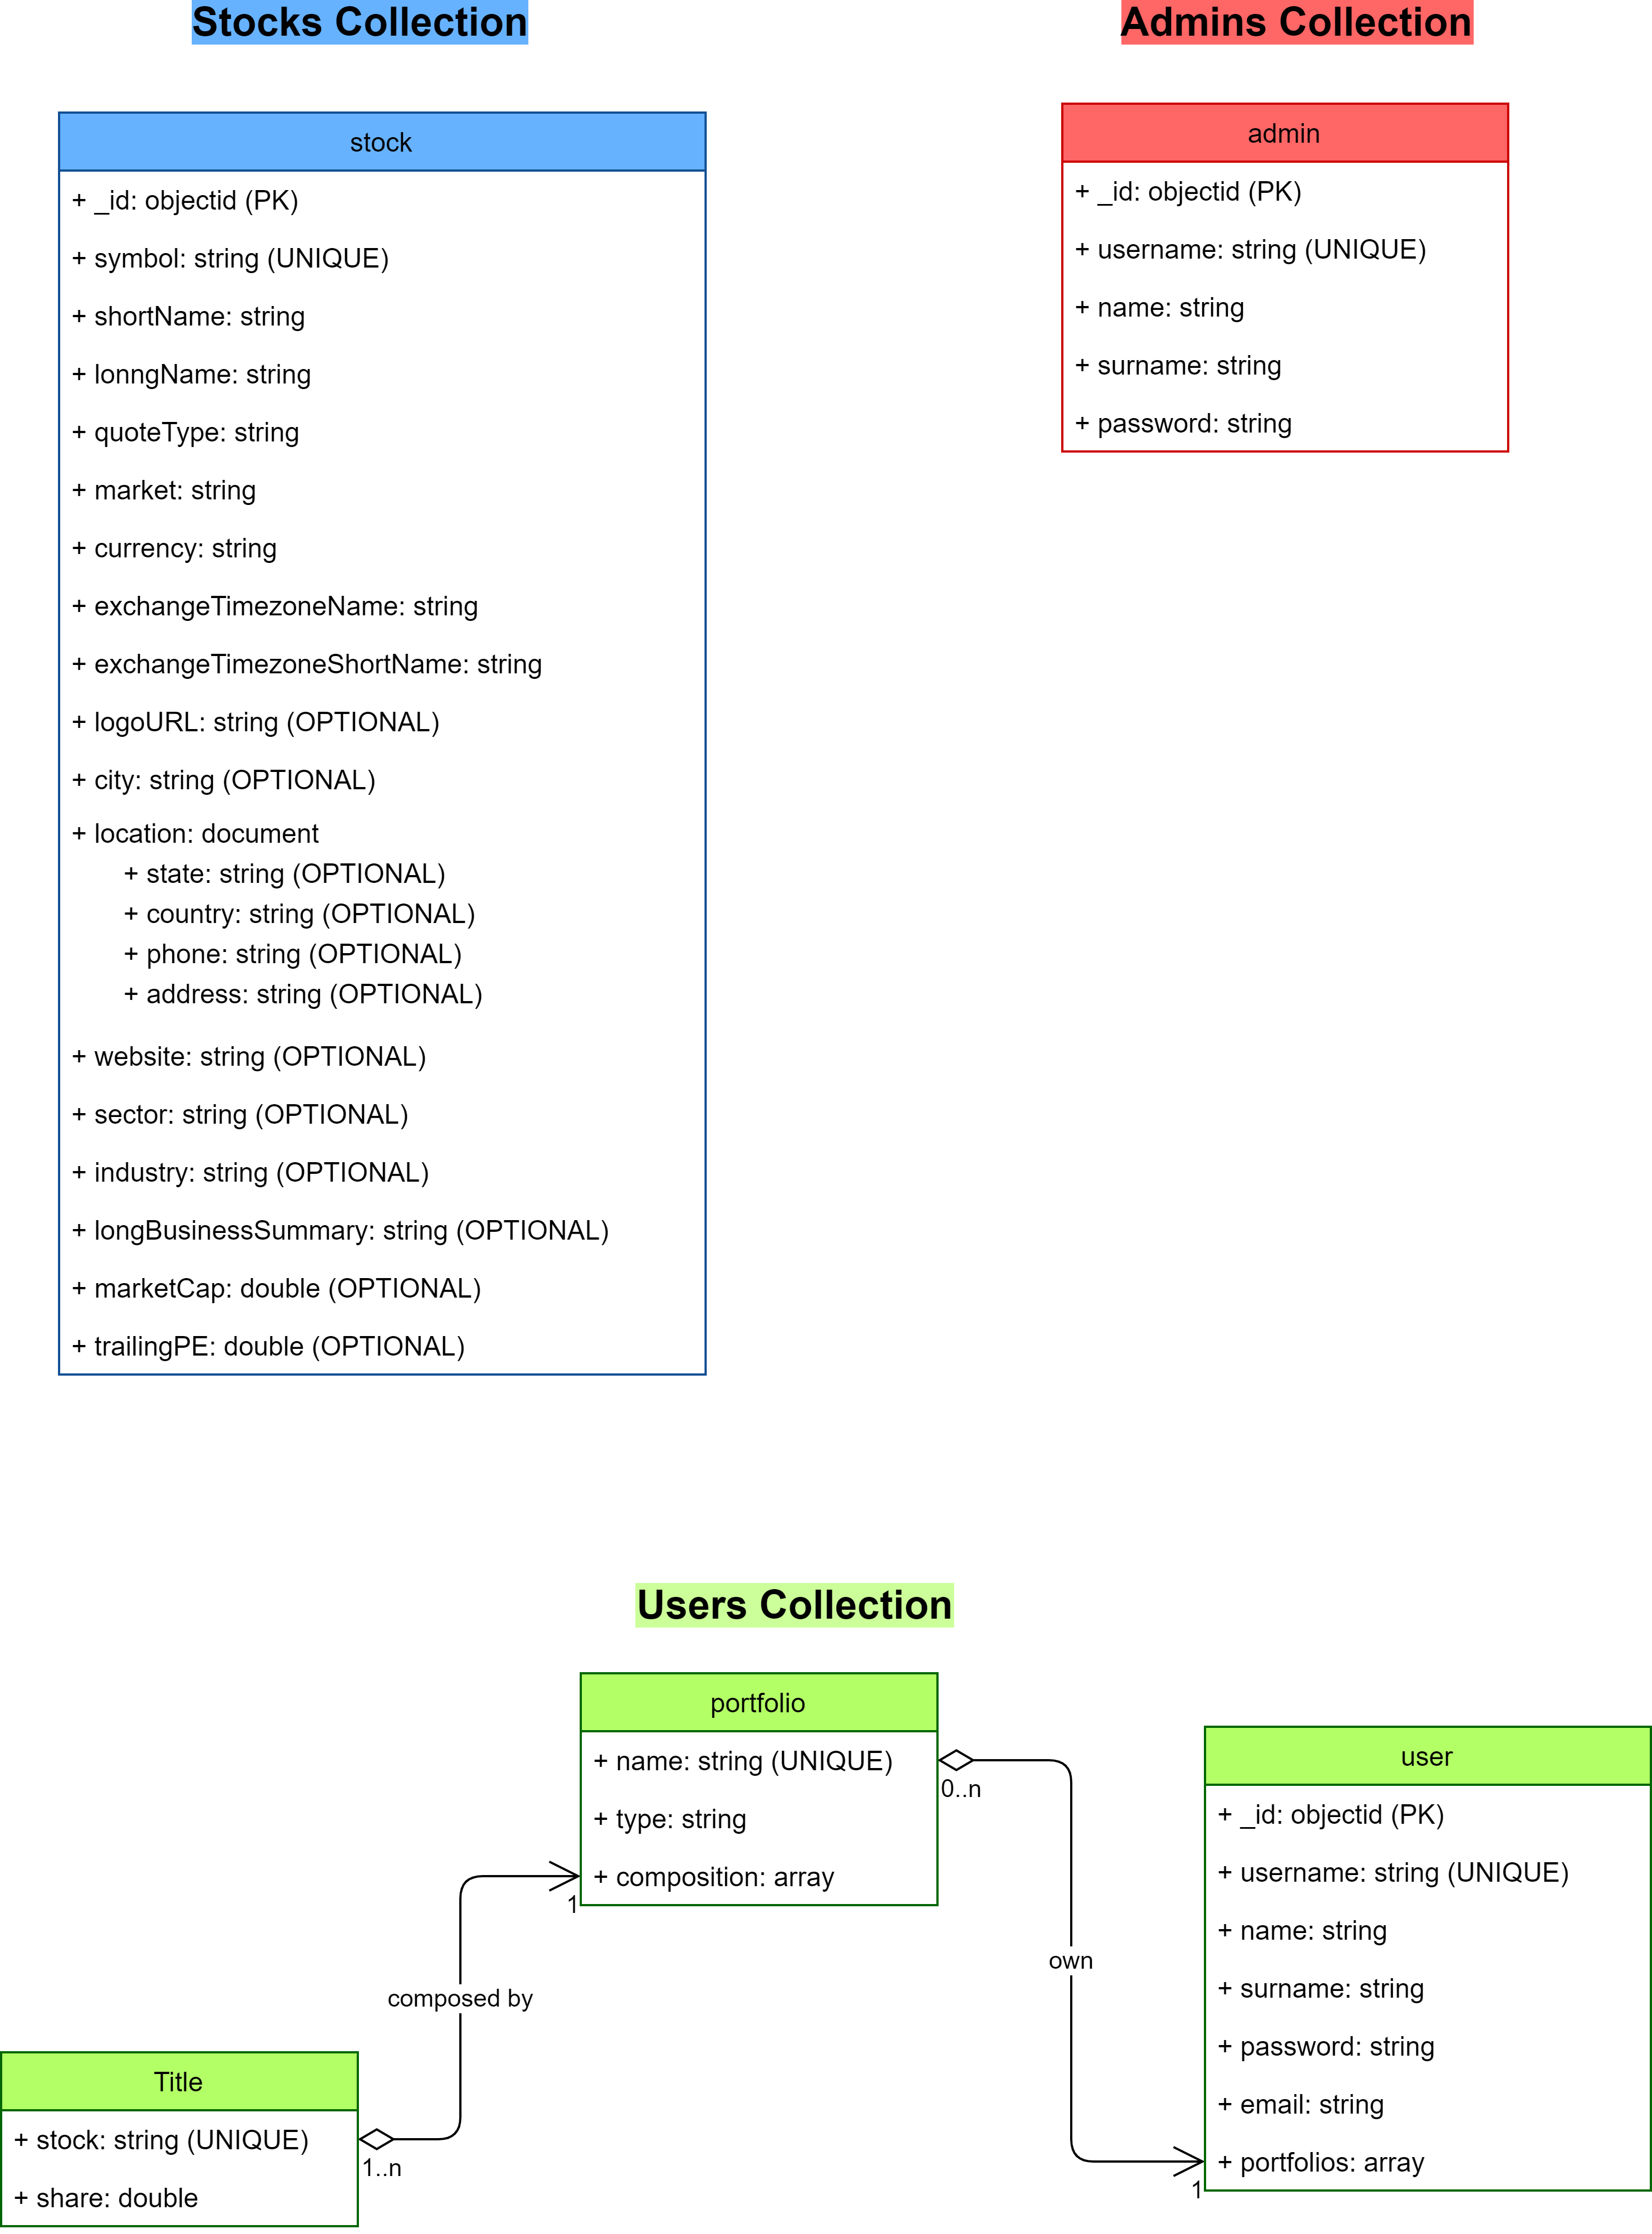
\includegraphics[scale=0.14]{img/mongoDB_schema.png}\\
}

\hfill \break
This scheme is composed by 3 collections: \textbf{stocks}, \textbf{users}, \textbf{admins};
\begin{itemize}
    \item
The stocks collection contains one document for each stock; inside this document
all the general information about the stock is stored; each stock is identified by the attribute SYMBOL.
Some basic information is always present, while other may be missing for some stocks; we decided 
to keep these last type of information were possible, exploiting the schemaless property of
the document database;
    \item
The \textbf{users} collection contains one document for each user registered on the application; in each of these documents, login credentials are stored, along with few personal information; for every user there is
also an array of documents named PORTFOLIOS: this array contains the portfolios of the user.
Each portfolio has a scheme, which includes an array of TITLEs, named COMPOSITION, which describes
what the portfolio consists of. This nested structure has been preferred over splitting
data in different collections, because all the information of a user, including their portfolios, 
is frequently needed at once; on the other hand, there are not operations that involve
portfolios owned by different users.
    \item 
The \textbf{admins} collection contains the admins login credentials together with few personal
informations about them; we decided to create a separated collection for administrators 
to improve the security of the administration features: in this way is impossible to inject
administration privileges through the login command.
\end{itemize}
\subsection{Aggregations}
One of the main features of our application is the possibility to choose some stocks from
the market and combine them into a portfolio. When a user is looking for a stock, they want to
know statistics about \textbf{industries} and \textbf{sectors}, along with classification by 
\textbf{level of capitalization} and  \textbf{PE ratio} (\textit{Price-Earnings Ratio}); in order to do so, we will provide
these aggregation pipelines:
\begin{itemize}
    \item the total market capitalization of each sector
    \item the total market capitalization of each industry
    \item the total market capitalization of stocks coming from the same country
    \item the average PE ratio of stocks working in the same sector
    \item the average PE ratio of stocks working in the same industry
    \item the average PE ratio of stocks coming from the same country
    \item the average PE ratio of stocks being in a specific range of market capitalization
\end{itemize}
We provide here an example of an aggregation Mongo query:
\begin{lstlisting}[basicstyle=\footnotesize,language=Java,numbers=left,
    numberstyle=\footnotesize,numbersep=4pt,frame=single]
    /**
    * Aggregates data with filtering and grouping by an attribute, can compute
    * sum, avg ecc.
    *
    * @param collection the collection where to perform the operation;
    * @param filter filter to be used to find the documents.
    * @param groupField the filed used to group the aggregation
    * @param aggregator the aggregator function and field
    *
    * @return iterable object containing the result of the aggregation.
    */
   public AggregateIterable<Document> aggregate(final Bson filter, final String groupField, final BsonField aggregator, final MongoCollection<Document> collection) {
       Bson match = Aggregates.match(filter);
       return  collection.aggregate(
               Arrays.asList(match, Aggregates.group("$"+groupField, aggregator)));
   }
\end{lstlisting}
\begin{lstlisting}[basicstyle=\footnotesize,language=Java,numbers=left,
    numberstyle=\footnotesize,numbersep=4pt,frame=single]
    MongoCollection<Document> collection1 = 
        dbManager.getCollection(
            StocksimCollection.STOCKS.getCollectionName()
        );
    // aggregate examples
    final Bson equity= eq("quoteType", "EQUITY"); //filter(s)
    // name of the field projected, field to accumulate
    // type of accumulation (sum, avg...)
    final BsonField marketCapAccumulator=Accumulators.sum("totalCap","$marketCap");
    AggregateIterable<Document> aggregateList =
                                        // grouping attribute
            dbManager.aggregate(equity, "sector", marketCapAccumulator, collection1);
    for (Document document : aggregateList) {
        System.out.println(document);
    }
    // avg example with nested attribute
    final BsonField PEAccumulator=Accumulators.avg("avgPE","$trailingPE");
    aggregateList =
            dbManager.aggregate(equity, "location.country",
                    PEAccumulator, collection1);
    for (Document document : aggregateList) {
        System.out.println(document);
    }
\end{lstlisting}
\subsection{Indexes}
In order to speed up read operation in the document database, 
we decided to introduce some custom indexes:
\begin{itemize}
    \item a REGULAR and UNIQUE index on the attribute \textbf{symbol} in the collection stocks;
    \item a REGULAR index on the attribute \textbf{marketCAP} in the collection stocks;
    \item a REGULAR index on the attribute \textbf{trailingPE} in the collection stocks;
    \item a REGULAR index on the attribute \textbf{sector} in the collection stocks;
    \item a REGULAR index on the attribute \textbf{industry} in the collection stocks;
    \item a REGULAR index on the attribute \textbf{country} in the collection stocks;
    \item a REGULAR and UNIQUE index on the attribute \textbf{username} in the collection users;
\end{itemize}
We provide some statistic that endorse our indexes choices\\

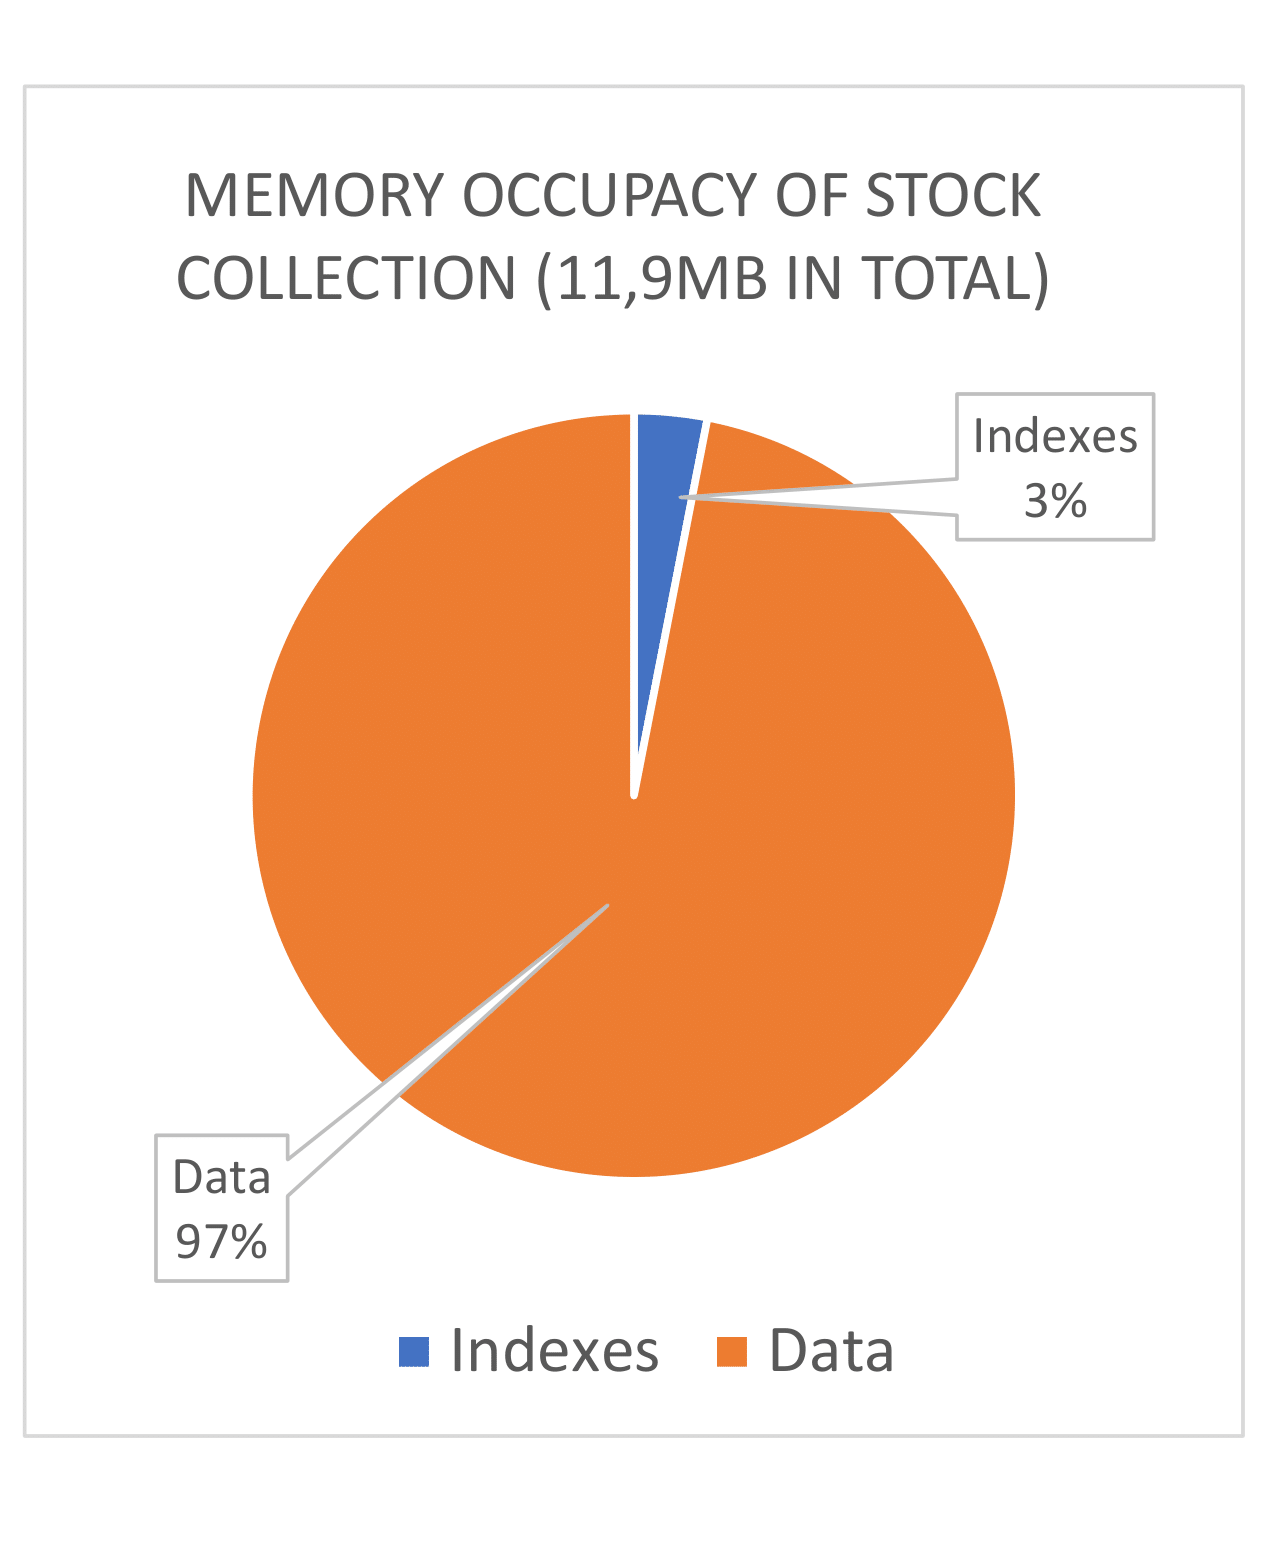
\includegraphics[scale=0.11]{img/memory_mongo.png}
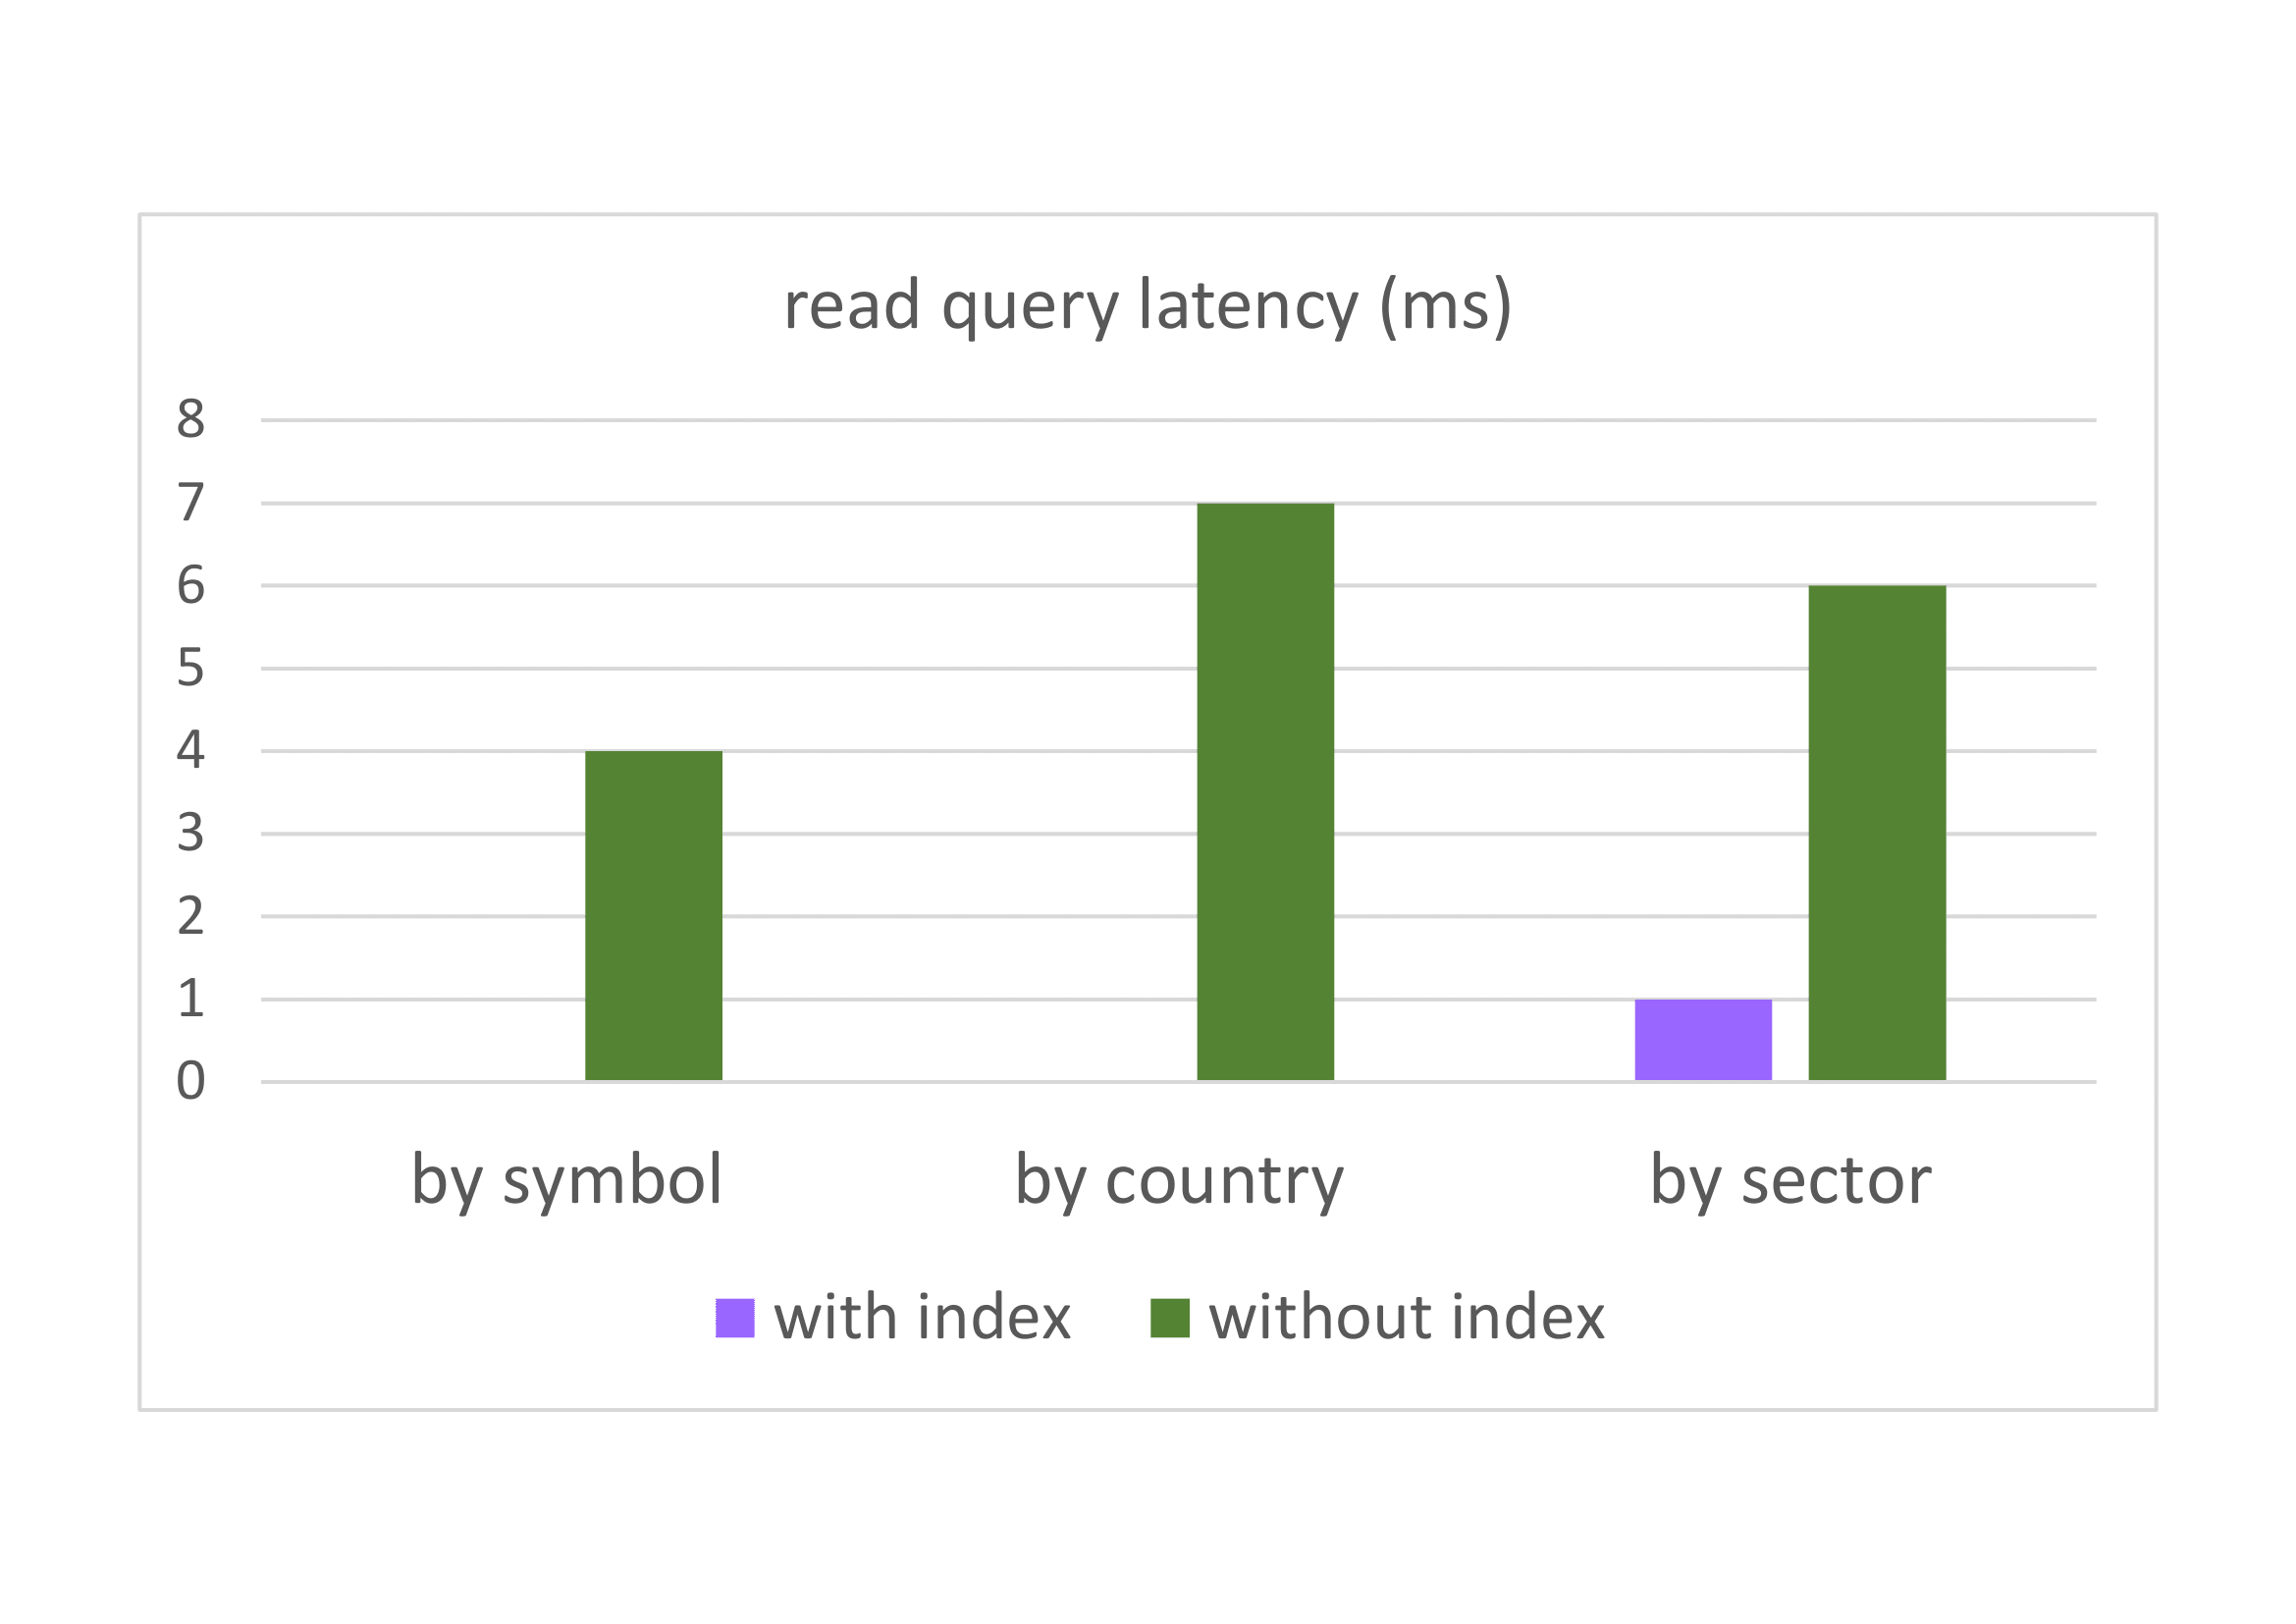
\includegraphics[scale=0.11]{img/latency_mongo.png}\\

\noindent Analog results can be found about the username index in the users collection.

\section{Apache Cassandra}
"The Apache Cassandra database is the right choice when you need scalability and high 
availability without compromising performance. Linear scalability and proven fault-tolerance 
on commodity hardware or cloud infrastructure make it the perfect platform for mission-critical 
data. Cassandra's support for replicating across multiple datacenters is best-in-class, 
providing lower latency for your users and the peace of mind of knowing that you can survive
regional outages." \footnote{https://cassandra.apache.org/}\\
Apache Cassandra is a database designed for high scalability and availability; it is 
capable to handle a huge amount of data and manage it in a decentralized architecture
across multiple nodes. It is built to be write optimized, but with the right indexes choices
read latency can be improved too; tables schemas and analytic functions can be customized.
This is the schema of our Cassandra database:\\
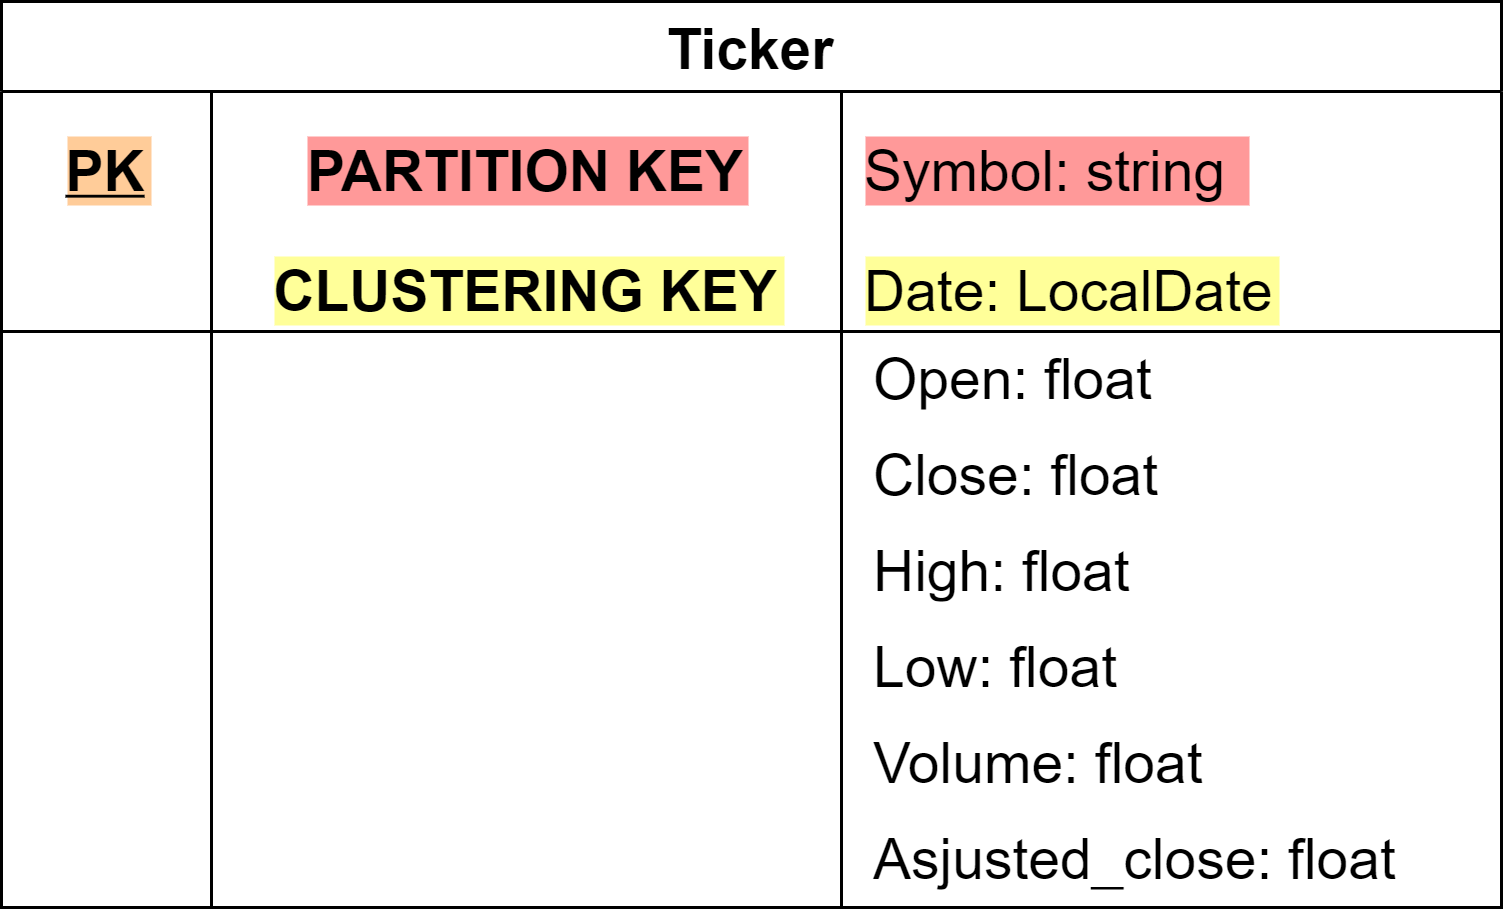
\includegraphics[scale=0.2]{img/cassandraDB_scheme.png}\\

\subsection{Aggregations}
In order to provide snapshots and statistics of stocks and portfolios trends over time,
we exploit the customization functionalities of Cassandra; a custom aggregation has been 
created, specifically to provide aggregate values for periods of time longer than one day; this allows us to obtain customizable granularity for stock market data,
computed on server side; this will not over overwhelm the server, because the aggregator will
execute, for each row, between a memory access and the following. This will greatly reduce
the data to be transmitted from the node to the client, saving bandwidth and time.  \\

\begin{lstlisting}[basicstyle=\footnotesize,language=SQL,numbers=left,
    numberstyle=\footnotesize,numbersep=4pt,frame=single]

    /* State function to be executed for every row*/
    CREATE OR REPLACE FUNCTION PeriodStateParam ( 

    /* the state, containing the aggregation result till this row */
        state map<date,frozen<map<text, float>>>,
    /*  the parameter ndays indicates the duration 
    *   of the period aggregation, in days          */
        ndays int, data date,  
        open float,  close float , high float,  low float, 
        volume float ,  adj_close float)
    CALLED ON NULL INPUT 
    RETURNS map<date,frozen<map<text, float>>> 
    LANGUAGE java AS '
    if (data != null) { 
        int d=0;
        Map<String, Float> statemap=null;
       
        for(d=1; d<ndays;){
            if((statemap=state.get(
                    data.add(Calendar.DAY_OF_MONTH,d)
                ))!=null)
                break;
            d++;
        }
        if(d==ndays){
            statemap=new HashMap<String, Float>();
            statemap.put("open", open);
            statemap.put("close", close);
            statemap.put("high", high);
            statemap.put("low", low);
            statemap.put("volume", volume);
            statemap.put("adj_close", adj_close);
            state.put(data,statemap);
        }
        else{
                if(high>statemap.get("high"))
                    statemap.replace("high", high);
                if(low<statemap.get("low"))
                    statemap.replace("low", low); 
                statemap.replace("volume",statemap.get("volume")+ volume);
                statemap.replace("open",open);
                state.replace(data, statemap); 
        }
    } 
    return state;'
     ;
    
    /*  aggregate declaration
    *   this aggregation generate a map data structure (JSON like):
    *   the key is the end date of each period of nday days, 
    *   and the value is another map containing the aggregate 
    *   values of the period as:
    *        the open of the first day
    *        the close and adjusted close of the last day
    *        the maximum of the highs
    *        the minimum of the lows
    *        the sum of the volumes
    */
    CREATE OR REPLACE AGGREGATE PeriodParam 
        ( int, date,float, float,float, float,float, float ) 
    SFUNC PeriodStateParam
    STYPE map<date,frozen<map<text, float>>>
    INITCOND {}; /* no initial condition is necessary */
    
    /* example of usage, it can be used also with grouping by symbol */
    select PeriodParam(
        20, date, open, close, high, low, volume, adj_close)
        as Period from tickers where 
        date<'2020-12-1' and date>'2020-6-10' 
        and symbol='TSLA';
    
\end{lstlisting}

\subsection{Indexes}
\begin{itemize}
    \item 
The PARTITION KEY index is part of the PRIMARY KEY and it is used to shard the dataset across
the nodes. This index is build on the string symbol, unique for each stock;
    \item
the CLUSTERING KEY i is also part of the PRIMARY KEY, and it is used to maintain rows in
chronological order. This index is built on the attribute date;
\end{itemize}
\section{Sharding and Replicas}
The MongoDB cluster and the Cassandra cluster are deployed on 3 virtual machines provided
by the University of Pisa; 
Our architecture is oriented to the availability of the service and built for the maximum
scalability and decentralization.
\begin{itemize}
    \item 
The Cassandra cluster is built among all 3 nodes, and data is sharded by ticker symbol;
in this way every node stores 1/3 of the main dataset, and aggregation functions are computed
on records that lie in the same node; each node also stores a backup of the data
assigned to another node, giving us a replication factor of 2. There are 2 seed nodes,
which are responsible for the cluster: the cluster is online as long as one of them keeps
working. This is indeed a minor issue, because in any case, with only one node, the dataset 
would by incomplete. The decentralized behaviour of Cassandra ensures that
even if all the node were to go offline, the cluster would return available as soon as one seed server went back
online. 
    \item
The MongoDB cluster is also built among all 3 virtual machines, and the service is replicated;
an initial primary server is elected, then another one will take its place if the former goes down. 
The cluster is available as long as one server is working, and incoming traffic could be balanced
with the "nearest" preference on client connection; in this way the client would connect to the
server with the lowest ping time.

\end{itemize}
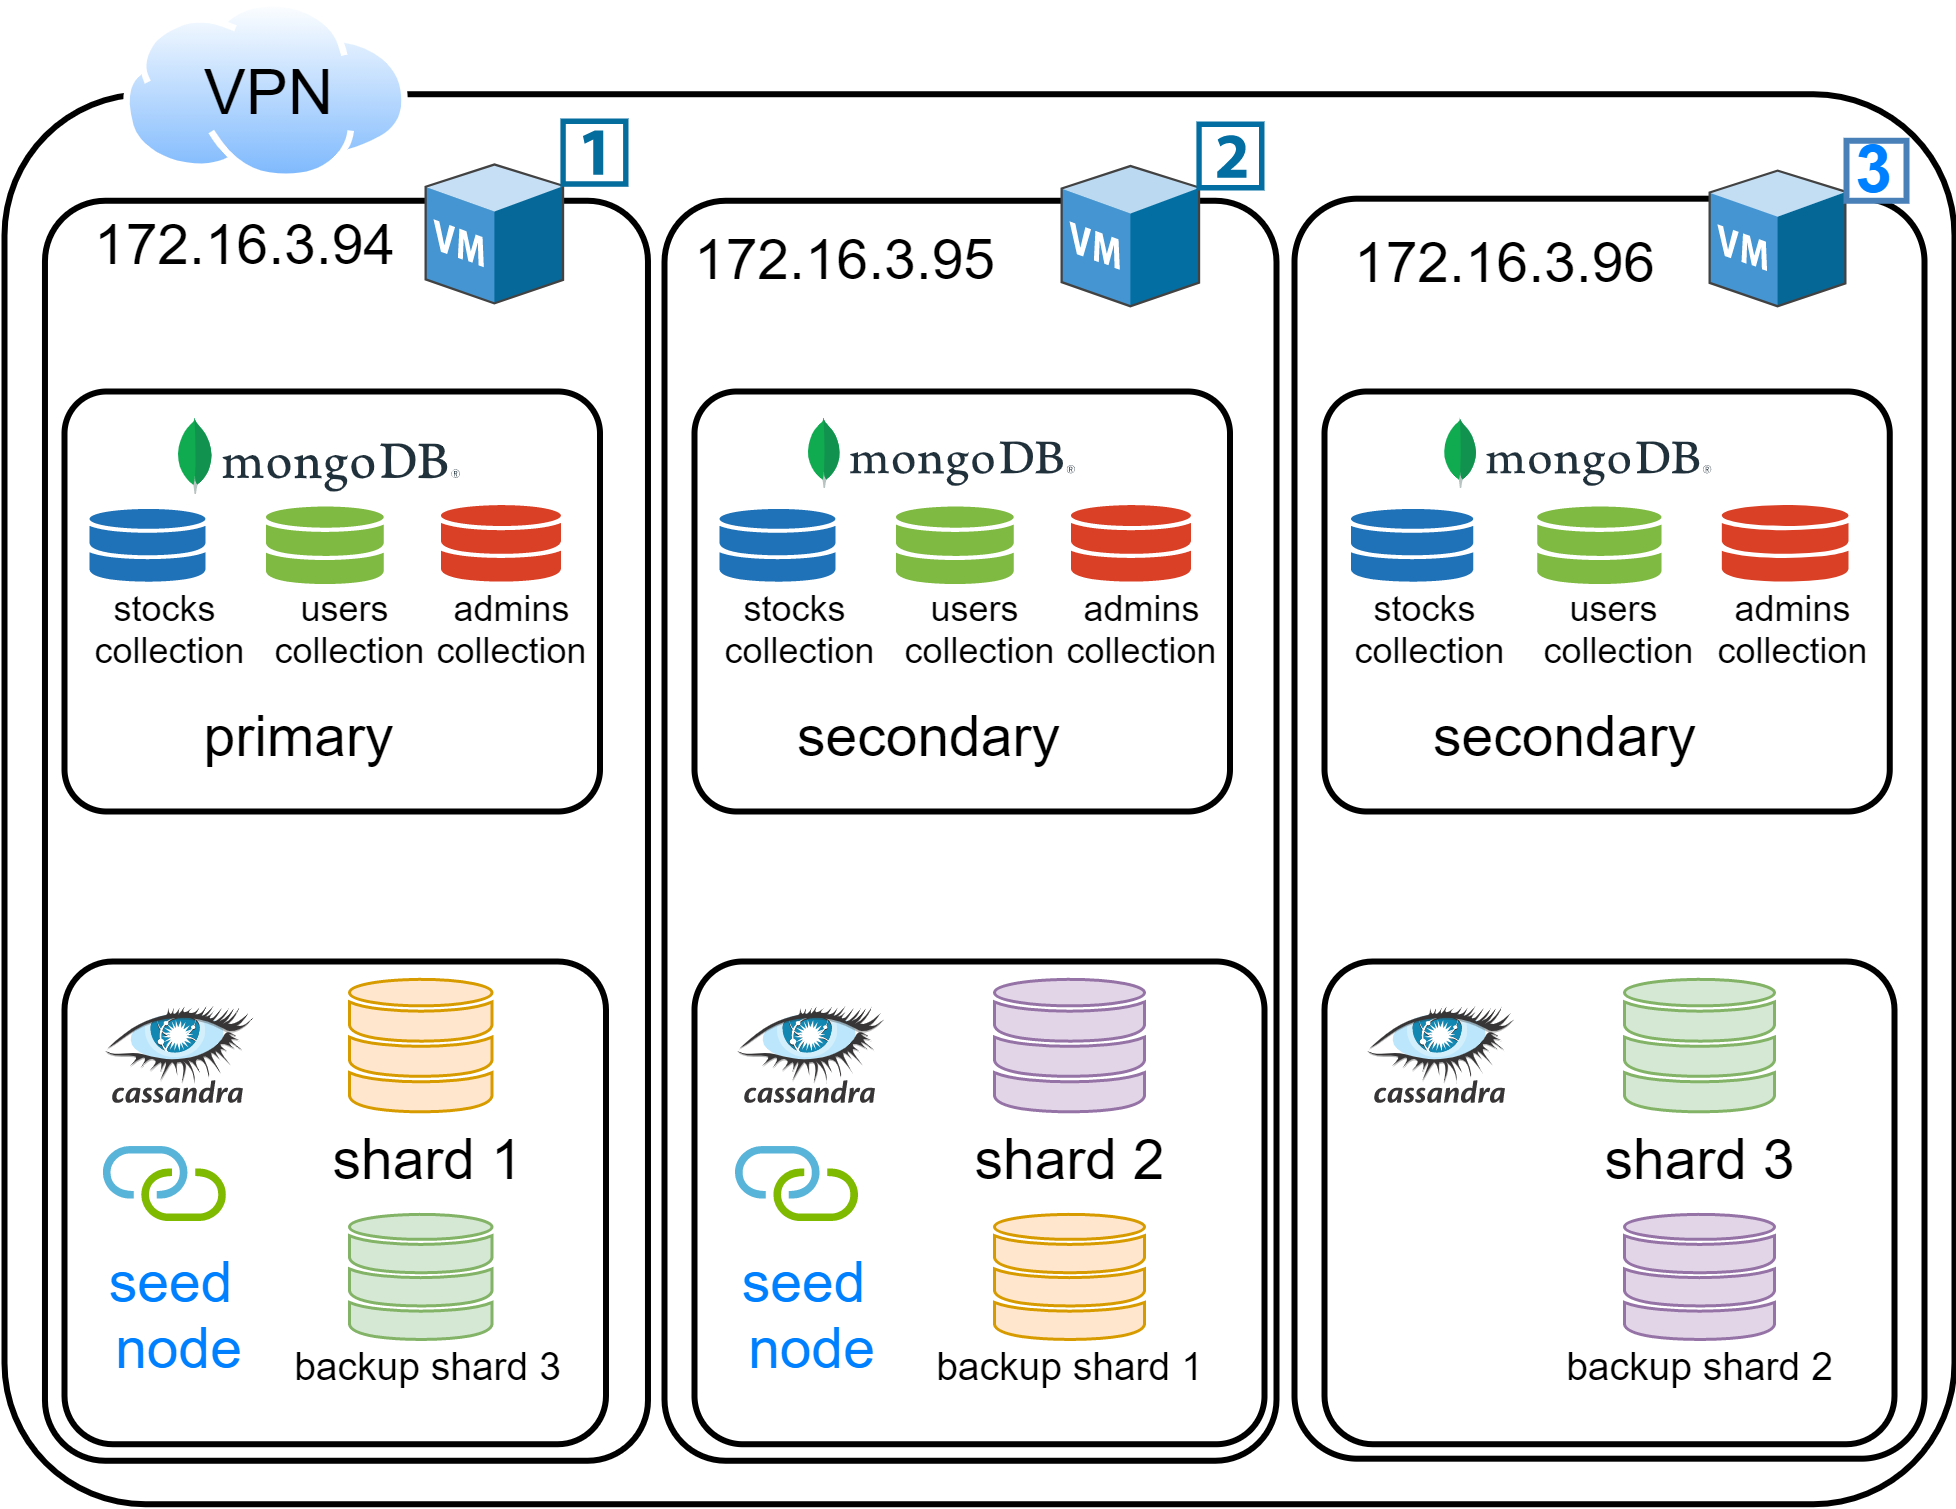
\includegraphics[scale=0.2]{img/cluster_diagram.png}\\
\section{Apache Cassandra vs MongoDB}
Cassandra and MongoDB are different database architectures but they share similar features. 
We know for sure that the usage of Cassandra can be avoided by adding a mongo Collection,
which can reproduce the behaviour of the Cassandra table for historical data. We want to explain
why in our opinion is better to store those data in Cassandra instead of Mongo, from a
performance and flexibility perspective.
\begin{itemize}
    \item 
    First of all, Cassandra has a native decentralized behaviour; we can't replicate all
    the historical data in every server, because hardware limitation, so we are forced to 
    shard data. Cassandra is specific designed for availability and partition tolerance,
    and can easy handle a node failure;
    \item 
    Cassandra can also compress data with advanced algorithms, which allow a node to store a lot
    of backup data from other nodes, increasing the availability of the service;
    \item
    Even if Mongo can store and aggregate our dataset in a decent way, the opportunity to
    create custom aggregation directly in Java language make Cassandra the best choice; this 
    allow us to perform every aggregation function that we need, and to add new ones;
    \item
    From a performance perspective, we ran the same query, on the same dataset, with the same 
    indexes structure, both in a Mongo collection and in our Cassandra keyspace; Cassandra
    always registered no latency, while mongo showed some ms of latency (4 in most cases);
    tests were performed on local storage, in the same machine,
    because remote latency performance would have been 
    somehow distorted by network swings.\\
    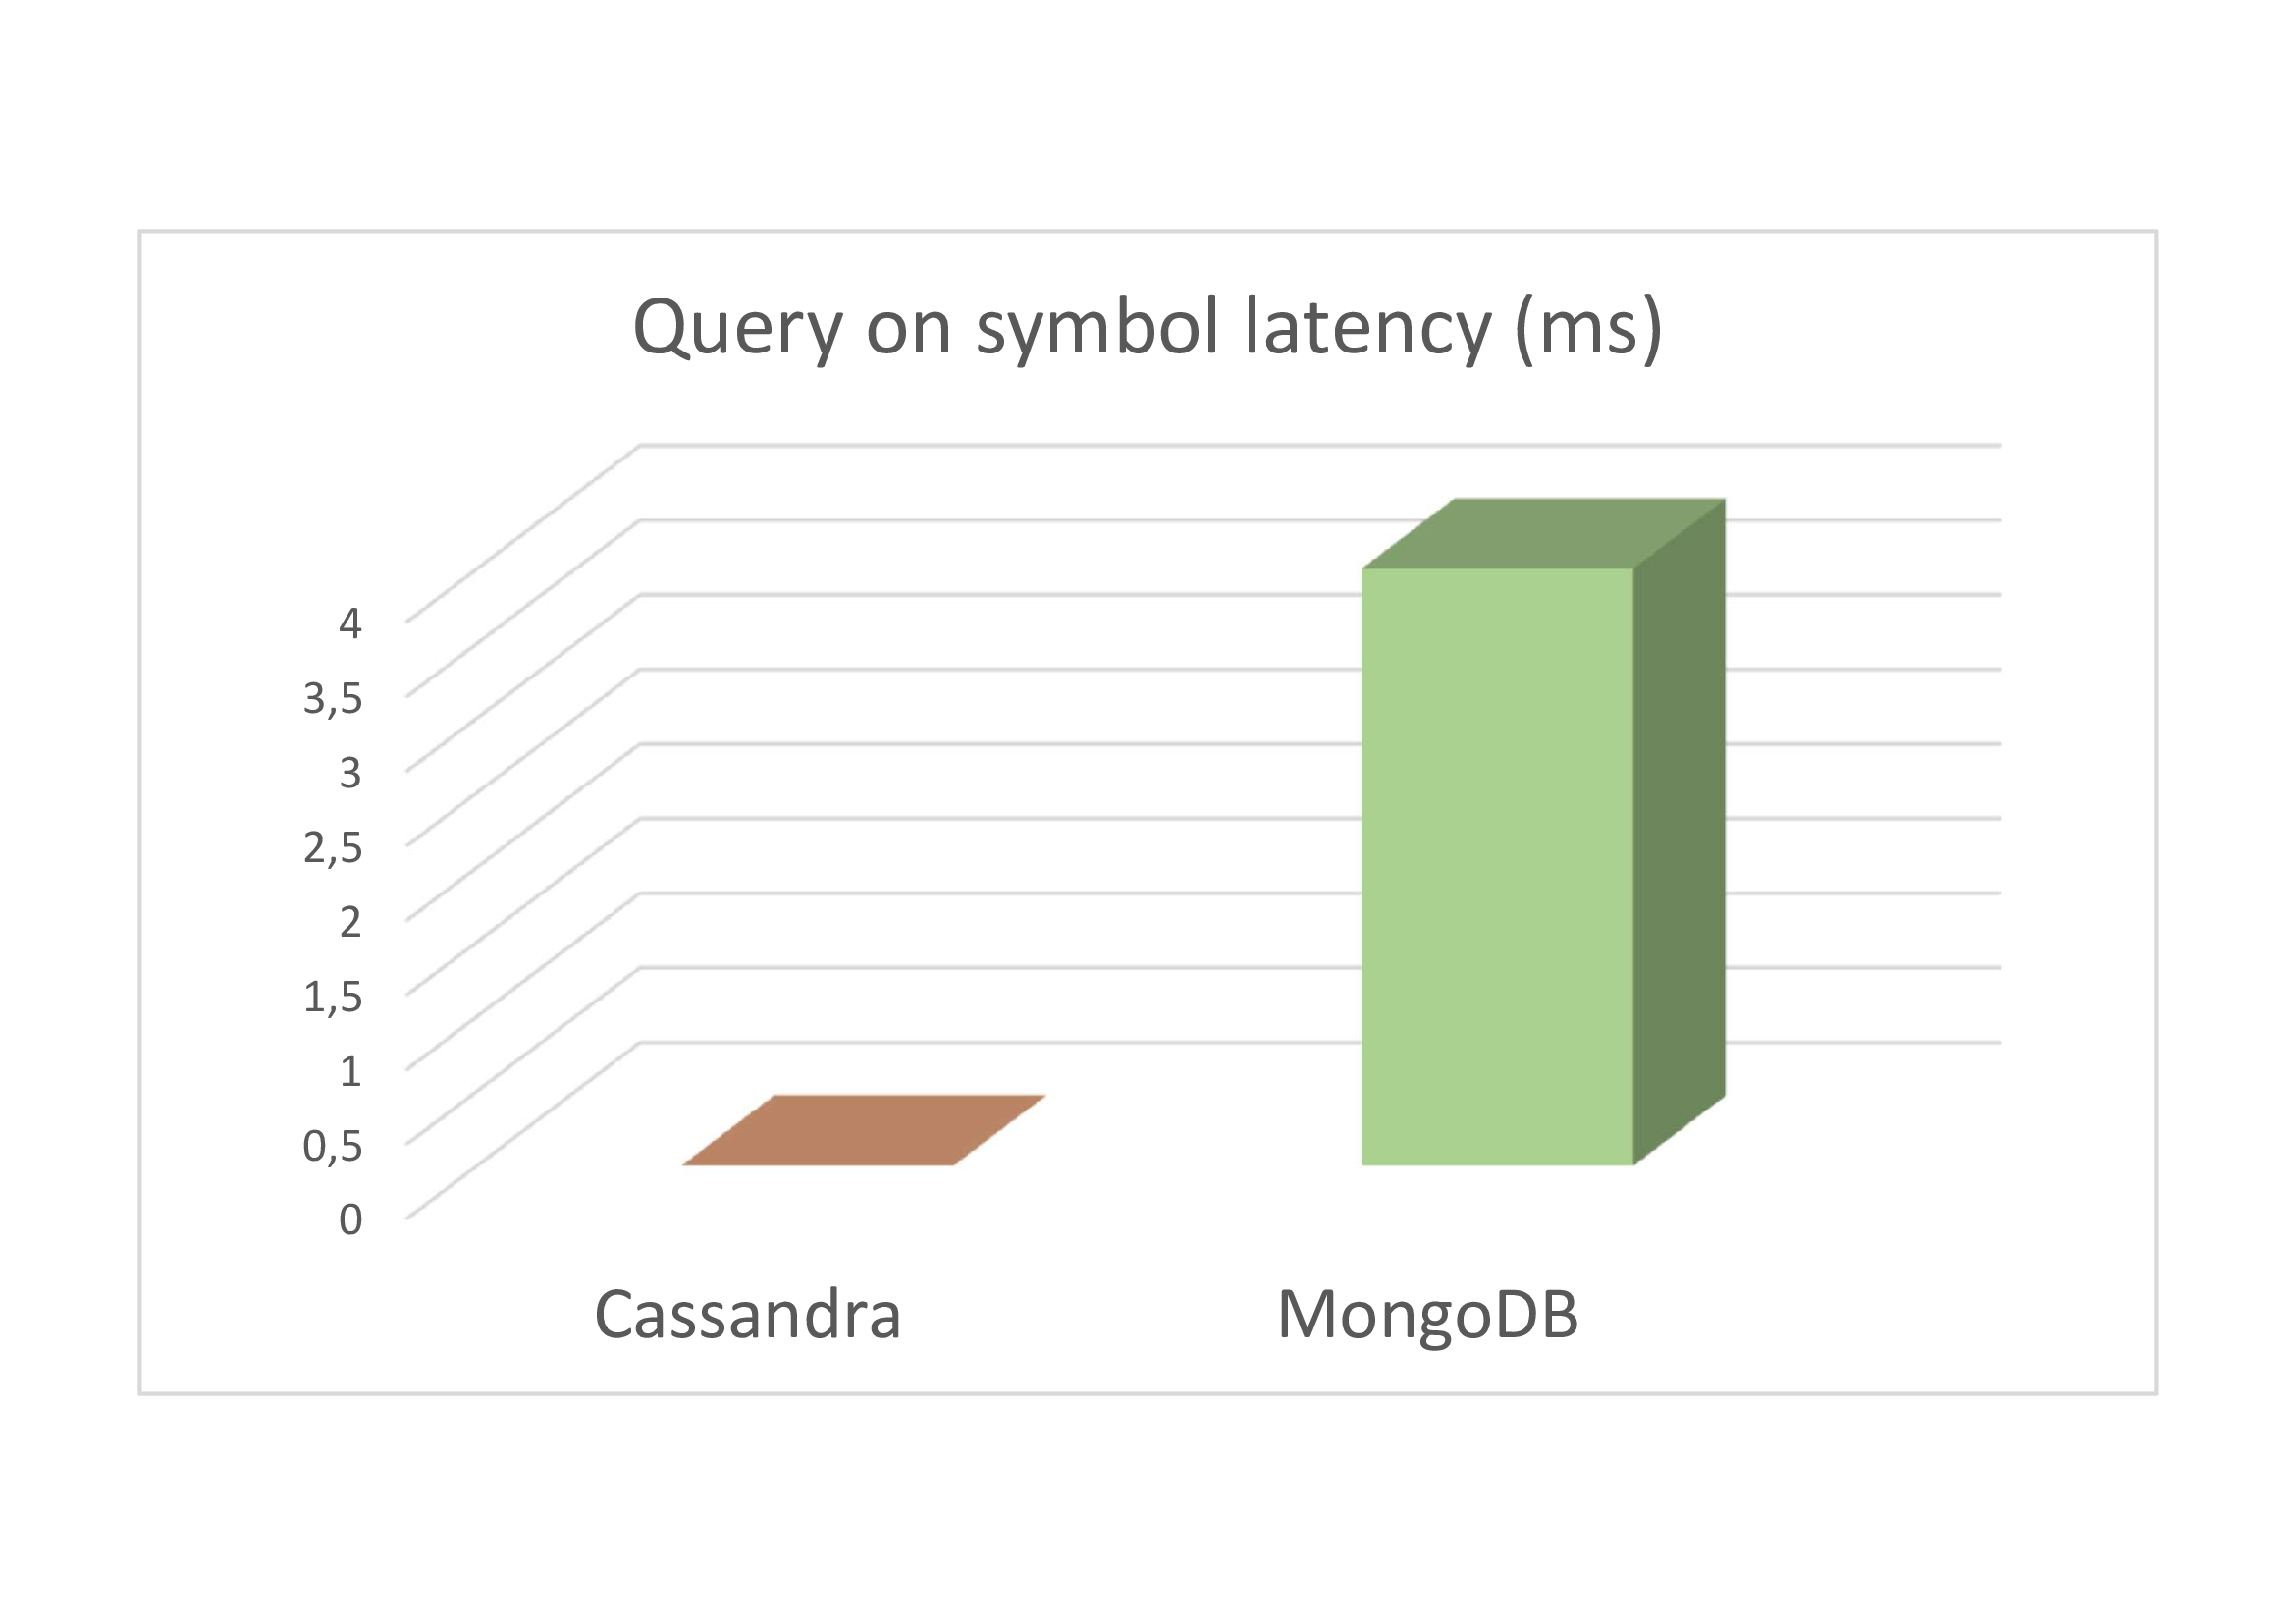
\includegraphics[scale=0.16]{img/cassandra_vs_mongoDB.png}\\

\end{itemize}